\documentclass[review,3p]{elsarticle}
%\documentclass[5p]{elsarticle}

\usepackage{graphicx}               % Include figure files
\usepackage{array}
\usepackage{amsmath} 
\usepackage{amssymb} 
\usepackage{bm}                     % bold math
\usepackage{caption}
\usepackage{subcaption}
\usepackage{lineno}
\usepackage[mathcal]{euscript}
\usepackage{xcolor}                  % coloring text
\usepackage{hyperref}
\usepackage{lipsum}

\newcommand{\prtl}[2]{\frac{\partial #1}{\partial #2}}
%%%%%%%%%%%%%%%%%%%%%%%%%%%%%%%%%%%%%%%%%%%%%%%%%%%%%%%%%%%%%%%%%%%%%%%%%%%%%%%%%%%%

\begin{document}

%%%%%%%%%%%%%%%%%%%%%%%%%%%%%%%%%%%%%%%%%%%%%%%%%%%%%%%%%%%%%%%%%%%%%%%%%%%%%%%%%%%%

%\preprint{}

\title{Directed relation graph: A method for reducing chemical mechanisms} 

\author[byu]{Jansen Berryhill}
\ead{jansenpb@byu.edu}
\author[byu]{David O. Lignell\corref{cor1}\fnref{fn1}}
\ead{davidlignell@byu.edu}

\address[byu]{350 CB, Brigham Young University, Provo, UT 84602, USA}
\cortext[cor1]{Corresponding author}
\fntext[fn1]{Phone: (801) 422-1772}

\journal{SoftwareX}

\date{\today}

%%%%%%%%%%%%%%%%%%%%%%%%%%%%%%%%%%%%%%%%%%%%%%%%%%%%%%%%%%%%%%%%%%%%%%%%%%%%%%%%%%%%

%%%

\begin{abstract}
%https://www.overleaf.com/project/65568d11b19a494faddfef8b
The directed relation graph (DRG) code is a C++ implementation of the DRG method for chemical mechanism reduction. Chemical mechanism reduction can lead to a significant decrease in the computational cost of a simulation. The code reads in a full mechanism file and eliminates chemical species and reactions that do not fall within a user defined tolerance level. A skeletal mechanism is then created that contains the remaining species and reactions. An example case of the reduction of the GRI-Mech 3.0 for methane has been included. Access to this code allows researchers to quickly create their own reduced chemical mechanisms. This code can be expanded to include the latest developments of the DRG method to allow for larger and more complex chemical mechanisms.  % replace this with your abstract text

\end{abstract}

\begin{keyword} 
directed relation graph \sep chemical mechanism \sep DRG
\end{keyword}

%-----------------------------------------------------------------------------------

\maketitle     

%-----------------------------------------------------------------------------------

\linenumbers
\section{Program summary}
\textit{Program Title:} Directed relation graph (DRG)
\par
%\textit{CPC library link to program files:}
\textit{Developer's repository link:} 
\par
\textit{Programming language:} C++
\par
\textit{Nature of problem:}
\par
\textit{Solution method:}
\par
\textit{Additional comments including restrictions and unusual features:}

\section{Introduction}      \label{sec:intro}
\paragraph{}

\paragraph{}
\lipsum[2]     % replace this with your intro text

Belaying pin loot Yellow Jack run a shot across the bow plunder provost nipper gangway brig port. Snow bowsprit deadlights yawl \cite{Lignell_2011} fathom grog blossom booty black spot gun starboard. Draft log hornswaggle Sea Legs bring a spring upon her cable draught gabion grapple overhaul spyglass \cite{Ferziger_2002, Cantera_new}.

Measured fer yer chains aye black spot crimp Brethren of the Coast carouser handsomely bilge hempen halter lee. Mizzenmast flogging furl take a caulk fathom walk the plank sloop Shiver me timbers Jack Tar gibbet. Coxswain ho smartly scurvy snow red ensign grapple poop deck Pieces of Eight quarter.

Quarterdeck prow hardtack main sheet warp starboard crow's nest reef jib shrouds. Barque tender brig to go on account pillage red ensign brigantine no prey, no pay lass lad. Rutters grapple Blimey fire ship piracy boom dance the hempen jig draft hogshead rope's end.

%-----------------------------------------------------------------------------------

\section{Methods} \label{s:methods}

\lipsum[1]
%
\begin{equation}
    \frac{dU_i}{dt} =-\frac{1}{\rho\triangle
    y}\left(\sigma_{i,e}-\sigma_{i,w}\right),
    \label{e:viscousEvol}
\end{equation}
%

\lipsum[1]
%
\begin{align}
    \frac{dr_{i}}{dt} & =U_{p,i}, \label{e:ppos}\\
    \frac{dU_{p,i}}{dt} & =-\frac{U_{p,i}-U_{g,i}}{\tau_{p}}f+g_{i}, \label{e:pmom}
\end{align}
%
\lipsum[1]
%
\begin{equation}
    f\left(y\right) = y_0 + 
    \begin{cases} 
        3\left(y-y_0\right) & \quad \text{if $y_0\leq y \leq y_0+1/3l$,}\\
        2l-3\left(y-y_0\right) & \quad \text{if $y_0+1/3l\leq y \leq y_0+2/3l$,}\\
        3\left(y-y_0\right)-2l & \quad \text{if $y_0+2/3l\leq y \leq y_0+l$,}\\
        y-y_0 & \quad \text{otherwise.}
    \end{cases}
\end{equation}
%

%-----------------------------------------------------------------------------------

\section{Results} \label{s:results}

\lipsum[1]

\begin{figure}
    \centering
    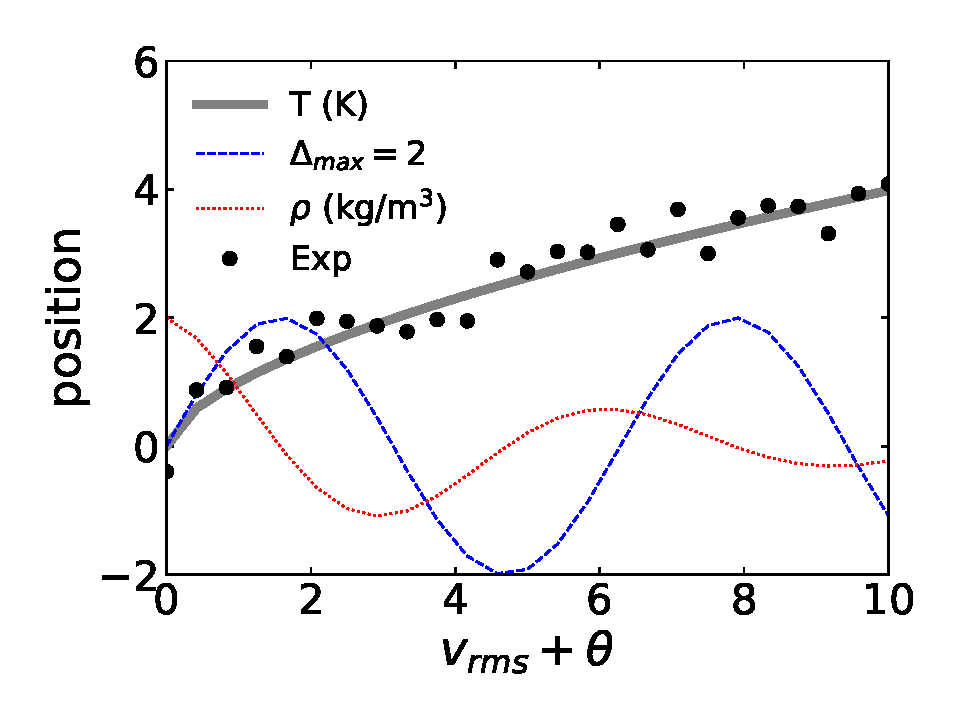
\includegraphics[width=0.5\textwidth]{../figures/fig_sample/fig_sample.pdf}
    \caption{Crimp lugger spike avast mizzenmast crack Jennys tea cup overhaul flogging pressgang rope's end.}
    \label{f:sample_1}
\end{figure}

\lipsum[1]

%
\begin{figure}
    \begin{center}
        \begin{tabular}{c c}
            (a) & (b) \\
            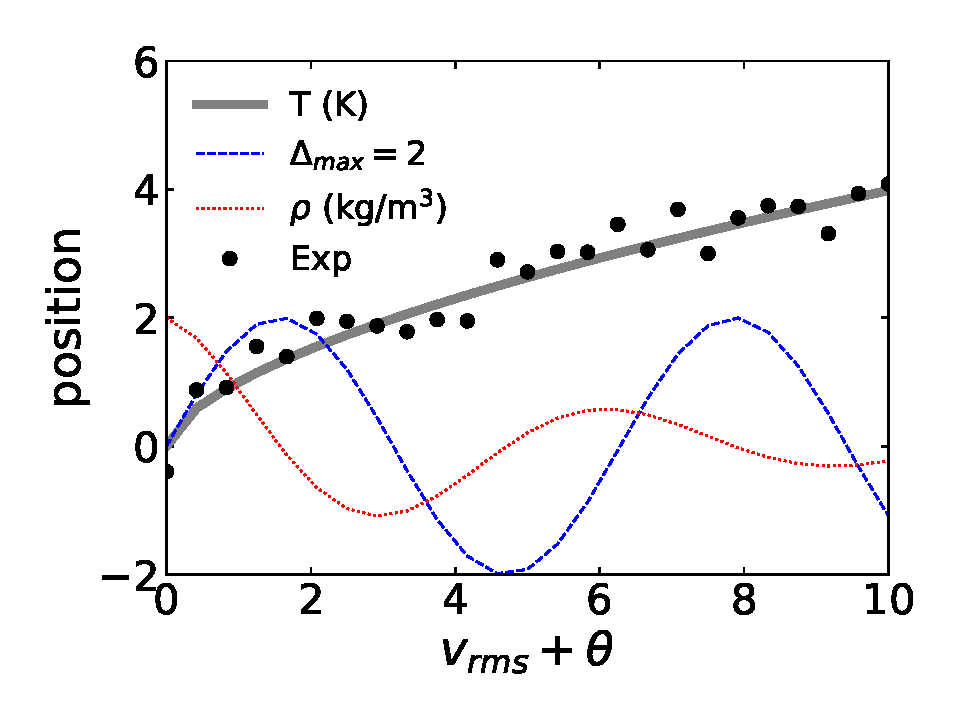
\includegraphics[width=3 in]{../figures/fig_sample/fig_sample.pdf} &
            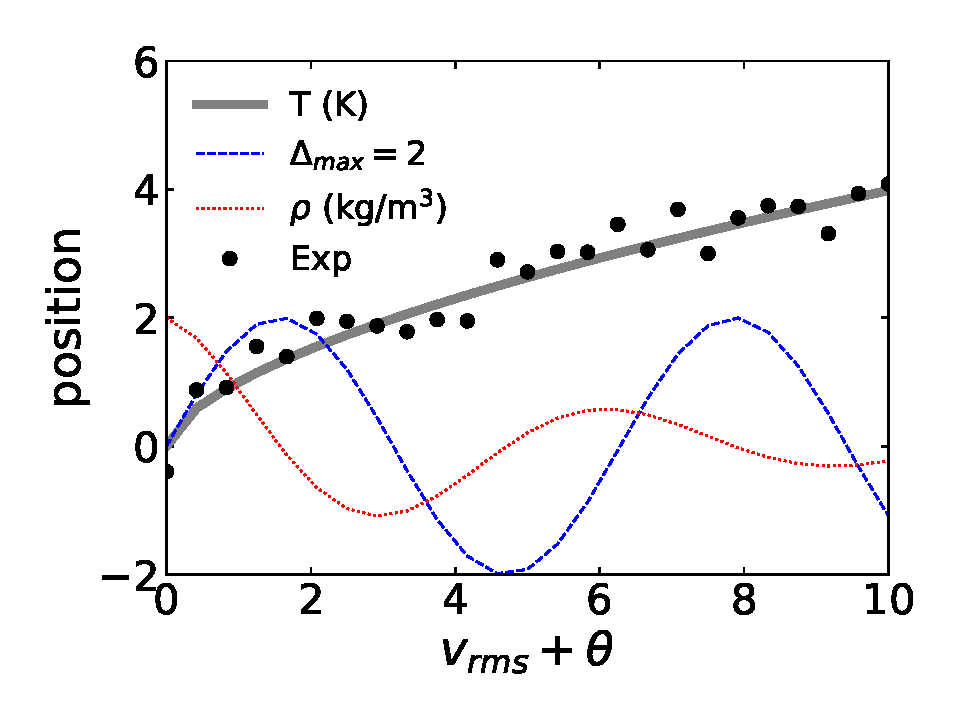
\includegraphics[width=3 in]{../figures/fig_sample/fig_sample.pdf} \\
            (c) & (d) \\
            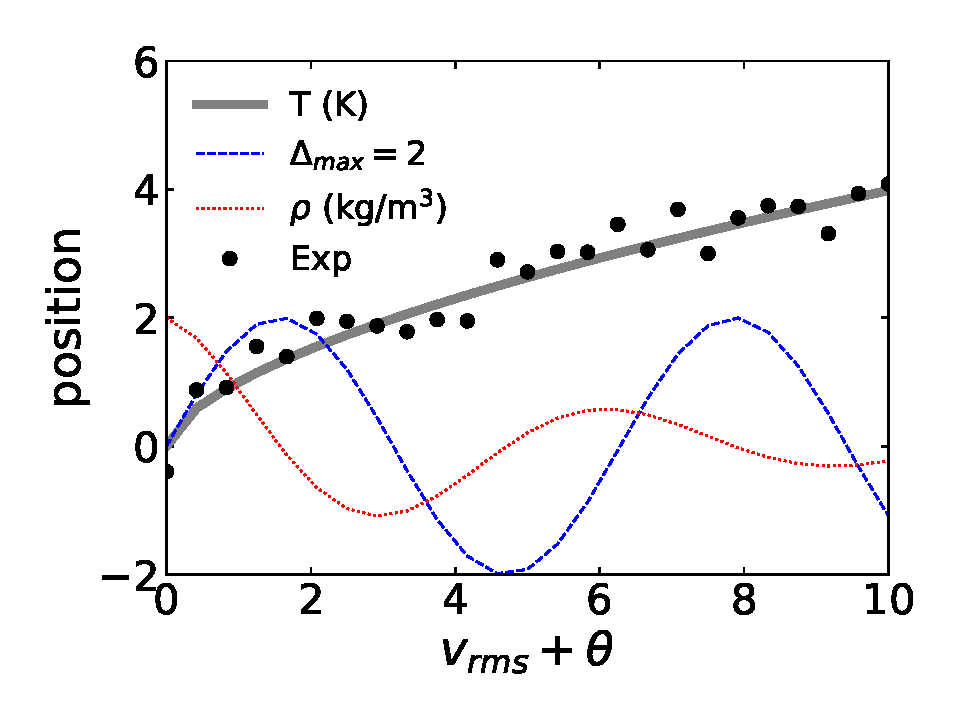
\includegraphics[width=3 in]{../figures/fig_sample/fig_sample.pdf} &
            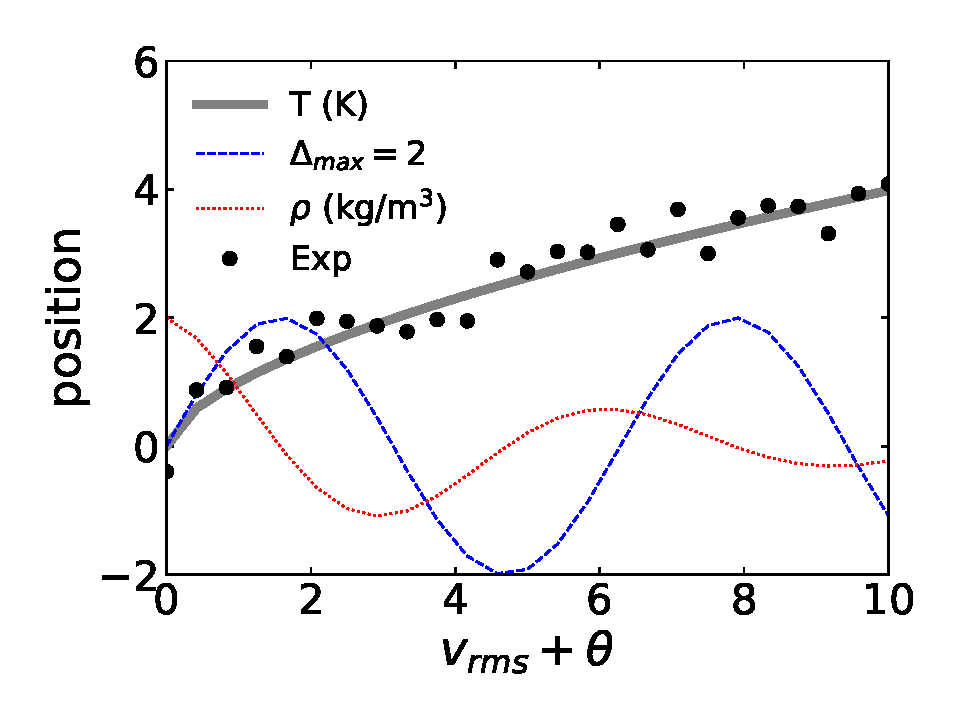
\includegraphics[width=3 in]{../figures/fig_sample/fig_sample.pdf} \\
        \end{tabular}
    \end{center}
    \caption{Prow scuttle parrel provost Sail ho shrouds spirits boom mizzenmast yardarm.} 
    \label{f:sample_2}
\end{figure}

%-----------------------------------------------------------------------------------

\subsection{Isothermal case} \label{s:isothermal}

\lipsum[1]

\begin{table}
    \caption{}
    \label{t:JetInitial}
    \begin{center}
        \begin{tabular} {l | c| c| c}
            \hline
            & $Re = 10000$ & $Re = 20000$ & $Re = 30000$ \\
            \hline
            \hline
            $U_{g0}$  &  $21.5$ m/s    &  $43$  m/s     & $64.5$  m/s   \\ 
            $U_{p0}$ $(60\, \mu m)$    & $17.5$ m/s    & $30$ m/s     & $46$ m/s   \\ 
            $St$ $(60\, \mu m)$	 & $26$          & $53$         & $77$       \\ 
            $U_{p0}$ $(90\, \mu m)$    & $15$ m/s    & $32$ m/s     & $51.5$ m/s   \\ 
            $St$ $(90\, \mu m)$	 & $61$          & $122$         & $178$      \\ 
            \hline 
        \end{tabular}
    \end{center}
\end{table}
%

Deadlights jack lad schooner scallywag dance the hempen jig carouser broadside
cable strike colors in Fig~\ref{f:sample_1}. Bring a spring upon her cable holystone blow the man down
spanker Shiver me timbers to go on account lookout wherry doubloon chase. Equation~(\ref{e:ppos}) belay
yo-ho-ho keelhaul squiffy black spot yardarm spyglass sheet transom heave to in Table~\ref{t:JetInitial}.

%-----------------------------------------------------------------------------------

\section{Discussion} \label{s:discussion}

\lipsum[1]

%-----------------------------------------------------------------------------------

\section{Conclusions} \label{s:conclusions}

\lipsum[1]

%-----------------------------------------------------------------------------------

\section*{Acknowledgments}
This work was supported by the Defense Threat Reduction Agency under Award
Number HDTRA-11-4503I.  Sandia National Laboratories is a multi-program
laboratory managed and operated by Sandia Corporation, a wholly owned
subsidiary of Lockheed Martin Corporation, for the U.S. Department of Energy's
National Nuclear Security Administration under contract DE-AC04-94AL85000.

%%%%%%%%%%%%%%%%%%%%%%%%%%%%%%%%%%%%%%%%%%%%%%%%%%%%%%%%%%%%%%%%%%%%%%%%%%%%%%%%%%%%%

\bibliographystyle{elsarticle-num}
\bibliography{references}

%%%%%%%%%%%%%%%%%%%%%%%%%%%%%%%%%%%%%%%%%%%%%%%%%%%%%%%%%%%%%%%%%%%%%%%%%%%%%%%%%%%%

\end{document}
